\question Imagine the map of the Bay Area as an undirected graph. We only have one day to explore the Bay but so many places to see. Find our shortest path tree with SFO airport as our starting point to visit every location on the map. (Edge weights are \underline{not} to scale). Resolve any ties alphabetically.
\setlength\parskip{1em plus 1pt}

\begin{center}
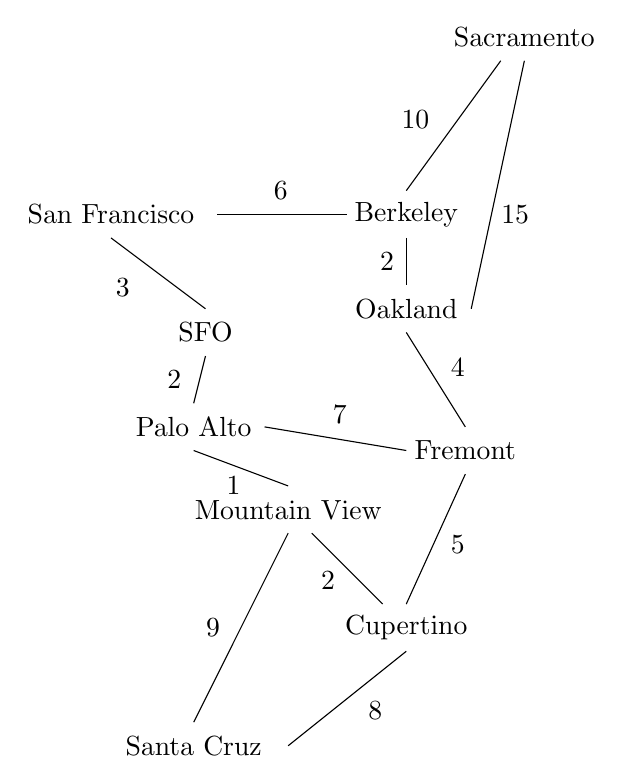
\begin{tikzpicture}[scale=0.15]
\tikzstyle{every node}+=[inner sep=0pt]
\draw (25,-15) node {San Francisco};
\draw (50,-15) node {Berkeley};
\draw (50,-23) node {Oakland};
\draw (33,-25) node {SFO};
\draw (60,0) node {Sacramento};
\draw (32,-33) node {Palo Alto};
\draw (40,-40) node {Mountain View};
\draw (32,-60) node {Santa Cruz};
\draw (50,-50) node {Cupertino};
\draw (55,-35) node {Fremont};

\draw (50,-13) -- (58,-2);
\draw (60,-2) -- (55.5,-23);
\draw (50,-17) -- (50,-21);
\draw (50,-25) -- (55,-33);
\draw (55,-37) -- (50,-48);
\draw (50,-52) -- (40,-60);
\draw (32,-58) -- (40,-42);
\draw (48,-48) -- (42,-42);
\draw (40,-38) -- (32,-35);
\draw (32, -31) -- (33,-27);
\draw (33,-23) -- (25,-17);
\draw (34,-15) -- (45,-15);
\draw (38,-33) -- (50,-35);

\draw (26,-22) node [above] {$3$};
\draw (52,-7) node [left] {$10$};
\draw (58,-15) node [right] {$15$};
\draw (49,-19) node [left] {$2$};
\draw (55,-43) node [left] {$5$};
\draw (48,-57) node [left] {$8$};
\draw (33,-50) node [right] {$9$};
\draw (44,-46) node [left] {$2$};
\draw (36,-38) node [left] {$1$};
\draw (31,-29) node [left] {$2$};
\draw (55,-28) node [left] {$4$};
\draw (40,-13) node [left] {$6$};
\draw (45,-32) node [left] {$7$};

\end{tikzpicture}
\end{center}

\begin{parts}
\part List vertices (locations) in the order in which they are dequeued (for the first time) from our priority queue and give the length of the shortest path from SFO airport.

SFO\hspace{.25cm}\rule{1cm}{0.15mm}\hspace{.25cm}\rule{1cm}{0.15mm}\hspace{.25cm}\rule{1cm}{0.15mm}\hspace{.25cm}\rule{1cm}{0.15mm}\hspace{.25cm}\rule{1cm}{0.15mm}\hspace{.25cm}\rule{1cm}{0.15mm}\hspace{.25cm}\rule{1cm}{0.15mm}\hspace{.25cm}\rule{1cm}{0.15mm}\hspace{.25cm}\rule{1cm}{0.15mm}

\hspace{.25cm}0\hspace{.3cm}\hspace{.25cm}\rule{1cm}{0.15mm}\hspace{.25cm}\rule{1cm}{0.15mm}\hspace{.25cm}\rule{1cm}{0.15mm}\hspace{.25cm}\rule{1cm}{0.15mm}\hspace{.25cm}\rule{1cm}{0.15mm}\hspace{.25cm}\rule{1cm}{0.15mm}\hspace{.25cm}\rule{1cm}{0.15mm}\hspace{.25cm}\rule{1cm}{0.15mm}\hspace{.25cm}\rule{1cm}{0.15mm}

\begin{solution}[.3in]
The order is:
\newline
SFO (0), Palo Alto (2), Mountain View (3), San Francisco (3), Cupertino (5), Berkeley (9), Fremont (9), Oakland (11), Santa Cruz (12), Sacramento (19)
\end{solution}

% \part Draw the edges with thick lines in the figure above.
% \begin{solution}[.5in]
% \begin{center}
% \begin{tikzpicture}[scale=0.15]
% \tikzstyle{every node}+=[inner sep=0pt]
% \draw (25,-15) node {San Francisco};
% \draw (50,-15) node {Berkeley};
% \draw (50,-23) node {Oakland};
% \draw (33,-25) node {SFO};
% \draw (60,0) node {Sacramento};
% \draw (32,-33) node {Palo Alto};
% \draw (40,-40) node {Mountain View};
% \draw (32,-60) node {Santa Cruz};
% \draw (50,-50) node {Cupertino};
% \draw (55,-35) node {Fremont};

% \draw (50,-13) -- (58,-2);
% \draw (50,-17) -- (50,-21);
% \draw (32,-58) -- (40,-42);
% \draw (48,-48) -- (42,-42);
% \draw (40,-38) -- (32,-35);
% \draw (32, -31) -- (33,-27);
% \draw (33,-23) -- (25,-17);
% \draw (34,-15) -- (45,-15);
% \draw (38,-33) -- (50,-35);

% \draw (26,-22) node [above] {$3$};
% \draw (52,-7) node [left] {$10$};
% \draw (49,-19) node [left] {$2$};
% \draw (33,-50) node [right] {$9$};
% \draw (44,-46) node [left] {$2$};
% \draw (36,-38) node [left] {$1$};
% \draw (31,-29) node [left] {$2$};
% \draw (40,-13) node [left] {$6$};
% \draw (45,-32) node [left] {$7$};

% \end{tikzpicture}
% \end{center}
% \begin{meta}
% Be sure to walk through this problem with your students. Be sure that they understand how ties are resolved and that we are using distance from SFO rather than edge weights to determine which the next point we add is.
% \end{meta}
% \end{solution}
% \vspace{1cm}\\
\part If every distance increased by 2 units (our car is old and slow \frownie), would our shortest path be the same?
\vspace{1.5cm}\\
% \hspace{1cm}\\
\begin{solution}
No it would not.
\begin{meta}
This is a bit of a trick question because this question may sometimes be yes depending on whether there are any cycles in the original graph to change the resulting tree if we add an amount to every edge weight. However, in this case, none of the cycles are affected by our increase in edge weights and even if we do add 2 to each weight, the resulting tree remains the same. Be sure to tell students that this answer depends on the graph and should be double checked with a quick mental walk-through of Dijkstra's.
\end{meta}
\end{solution}

\part What if we multiplied each weight by 10?
\begin{solution}
No change.
% \begin{meta}
% No matter what our graph looks like, a multiplicative factor to the edge weights will \underline{never} change the resulting tree using Dijkstra's.
% \end{meta}
\end{solution}
\end{parts}
